
\documentclass[main.tex]{subfiles}
\begin{document}

\begin{figure}
\caption{SEDA Software Architecture}
\centering
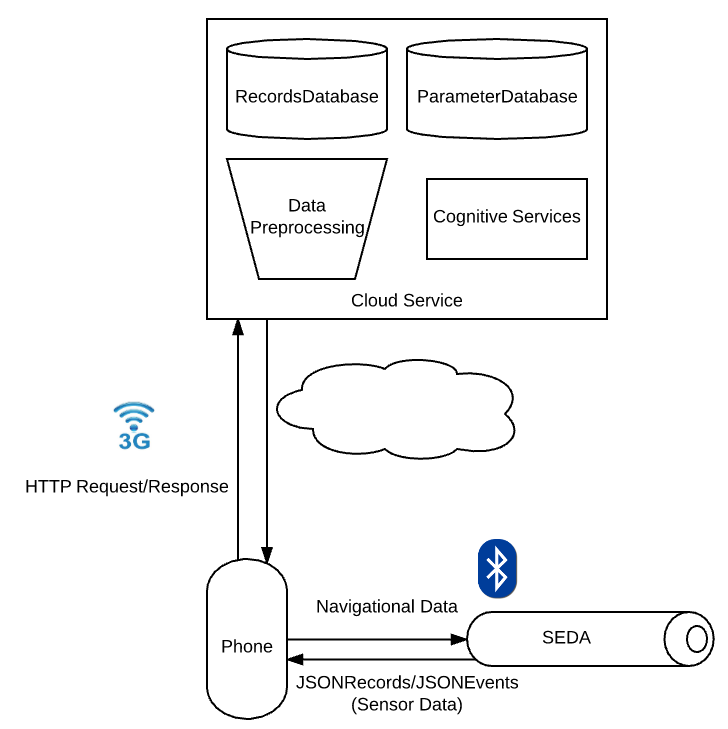
\includegraphics[width=\columnwidth]{SEDA_Architecture}
\end{figure}

\subsection{SEDA Application}


We aimed to build a lightweight device with long battery life. As the SEDA was attached to glass frame, we also minimized the computing power on the SEDA to reduce heat emission. So the software running in the SEDA was only capable for image recognizing jobs and senor data processing. Heavy computing tasks which required analyzing historical data were running at the server side.
\\
\\
\\
\\
\\

Main functions of the SEDA:

\textbf{Actively} gave real time advice and warnings to the user through speaker based on data acquired from senors, with pre-configured user profile. User profile contained the parameters for measuring safe driving. For example, the minimum car distance the user should keep under certain speed level. There were different sets of parameters stored in \emph{ParameterServer}, the user could choose to load their desired parameter set or default one as a profile. We adopted the algorithm from \cite{fang2004automatic} to detect vehicle through car plate matching, and along with \cite{alom2007road} detecting road signs by image pattern matching. These technologies existed for more than 10 years and prove to be efficient and effective. A study by the American Automobile Association (AAA) states that more than half of deadly crashes between 2003 and 2007 involved one or more unsafe driving behaviors typically associated with aggressive driving. We implemented DTW algorithms using gyroscope data which introduced in the paper \cite{johnson2011driving} to analyze the driver's behavior and give warning when aggressive driving was detected.

\textbf{Passively} collected data and uploaded to \emph{RecordDatabase}. Data were stored in JSON format and sent to database. There were two types of data: \emph{JSONRecords} and \emph{JSONEvents}. Data were uploaded automatically in a wireless environment. In the following session, we explain the JSON data structure the SEDA recorded to local memory.

\emph{JSONRecords}: snapshot the current state in every 2 seconds interval. Most of data from this record is generated from navigator. 
\\
\\
\\

\begin{figure}
\caption{JSONRecord collected from SEDA}
\centering
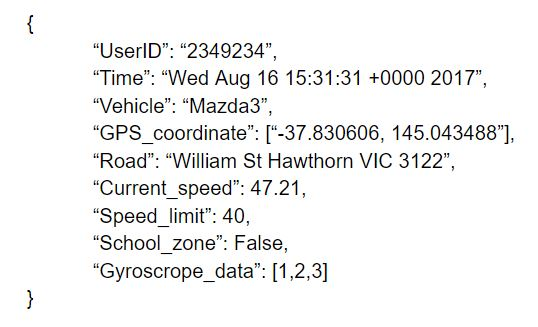
\includegraphics[width=\columnwidth]{json_record_1}
\end{figure}

\emph{JSONEvents}: these are triggered and stored when some events are encountered, which can potentially determine whether a driver has good driving habit or not. There could be more types of event recorded as SEDA learns.

Head check: records whether the driver made head checks in different scenarios.

\begin{figure}
\caption{Head check JSONEvent collected from SEDA}
\centering
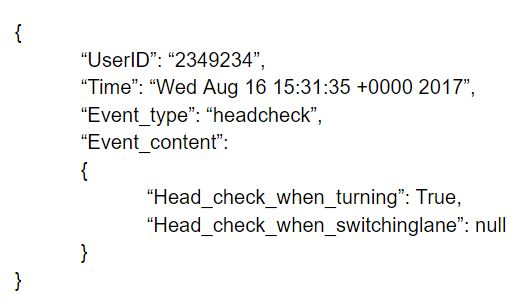
\includegraphics[width=\columnwidth]{json_event_1}
\end{figure}


Car Distance: if the measured minimal car distance is lower than the safety threshold at certain speed level, then car distance event is recorded.

\begin{figure}
\caption{Car distance JSONEvent collected from SEDA}
\centering
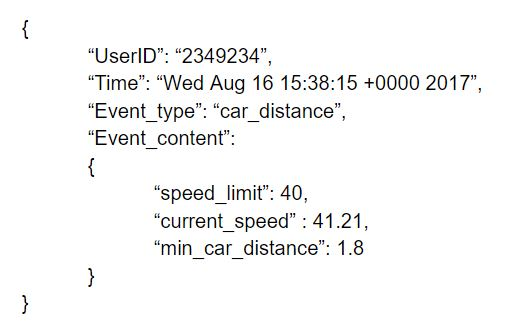
\includegraphics[width=\columnwidth]{json_event_2}
\end{figure}

\subsection{Mobile Application (Base App)}


Mobile application consists two parts:
One was GUI for accessing the \emph{RecordsDatabase} - User viewed their historical driving data and submitted requests for analysis. User can also configure their SEDA device in the user interface. 

When available, the smart phone GPS data together with navigational data such as GoogleMap streamed to SEDA for  current geographical location, road, speed limit. These information needed when generating \emph{JSONRecords} and \emph{JSONEvents}.



\subsection{Server Side Application}
 
Firstly, the server handled all the http requests from mobile phone. We used Kalman filter to prepossess the raw data and predefined algorithms to calculate the rating score of a driver within a certain period. This gave them a view of their historical data stored in database and showed the result and a brief report of analyzing users' past driving records. 

Additionally, the evolution of the SEDA system also happened in the server side program. It performed Big Data analytics on all users historical data, resulted in updating and perfecting the default profile in \emph{ParameterServer}. Such that the SEDA would perform better. For example, if car accidents happened  frequently in road abc, Server side program can use queries to get all recent records that a user drive along that particular road. Then analysis can be conducted to see the reason behind the car accident. Then the server will do parameter tuning to update the default profile. After the user updating the profile in configuration, they get warned when they are doing something similar actions that may cause accident.

\begin{figure}
\caption{SEDA Base App Mock UI}
%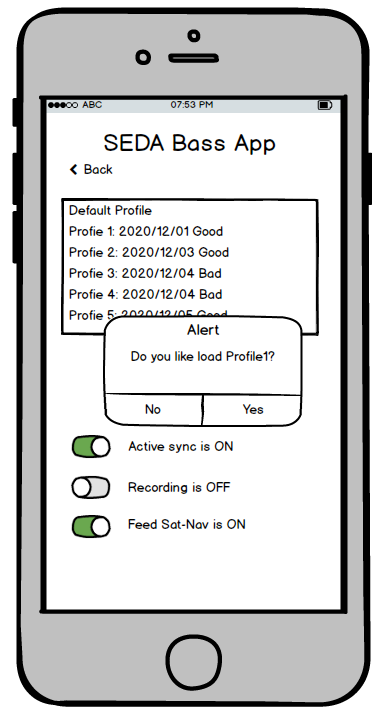
\includegraphics[width=\columnwidth]{seda_base_app}
\centering
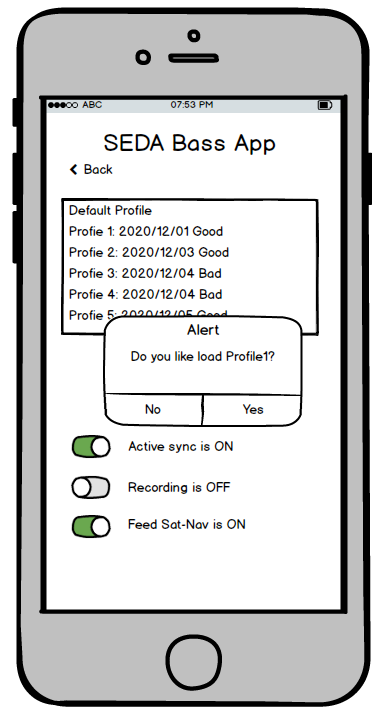
\includegraphics[scale=0.32]{seda_base_app}
\end{figure}


\end{document}